\documentclass[a4paper, twoside, 12pt]{report}
\usepackage[colorlinks=false,
allbordercolors={0 0 0},
pdfborderstyle={/S/U/W 1}]{hyperref}
\usepackage{mathtools}
\DeclarePairedDelimiter\abs{\lvert}{\rvert}%
\usepackage[margin= 1 in]{geometry}
\usepackage{graphicx}
\usepackage{caption}
\usepackage{subcaption} 
\graphicspath{ {images/} }
\usepackage{makecell}
\usepackage{float}

\begin{document}
\title{STA160 Project Report - Fake Twitter Account Detection}
\maketitle
\author{By: Tongke Wu, Guanyu Chen, Jieyi Chen}
{}
\section{Abstract}
%\\
As one of the most influential social networks in the world, Twitter is not only the showcase of people's daily life but also the channel of news and public opinions. The individuals can rise to fame through their tweets' popularity while the entities could encounter major crisis if their scandals are tweeted. Meanwhile, people have used fake accounts to produce tweets and comments to inflate the popularity of certain users and particular topics. Therefore, it is crucial to develop a model to discover the current fake Twitter accounts so that the public is aware of their influences.\\

\noindent In this paper, we create 45 features to analyze each Twitter account and apply these information to develop random forest, logistic regression and support vector machine models to discriminate between genuine and fake accounts.

\section{Introduction}
According to a study done by the University of Southern California and Indiana University, there are approximately 9 - 15\% Twitter active monthly users are bots, which is around 28.9 million to 47.9 million potential fake users[1] . Therefore, the twitter users will be the major beneficiary of our project results because they want a tool to help them identify whether the account is fake. 

\section{Data/Source}
First, we got Twitter accounts dataset from \href{http://mib.projects.iit.cnr.it/dataset.html}{My Information Bubble}. Then, we used the labeled accounts provided by this website to get user profile, tweet and follower information from the Twitter API. Some limitations that we encountered was the Twitter API's rate limits, in which we can only make 1 requests per 15 minute periods. In addition, we can only retrieve a maximum of 3,200 possible tweets for one user.\\

\noindent To evaluate the authenticity of a twitter account, we randomly selected 3250 accounts from our original dataset that contains 11151 users three times. Each sample data set includes approximately 90\% genuine accounts and 10\% fake accounts because we want to mimic the distribution in reality.

\section{Features}
\subsection{Profile-based Feature}
* Number of followers\\
\noindent* Number of tweets\\
\noindent* Fo-fo ratio: the ratio of the number of an account's following to its followers\\
\noindent* Age of the user account [2]\\
\noindent* Reputaion score\\
\noindent* Following choice: $F=\frac{T_n}{D_n}$ where $T_n$ is the total number of names among the account's followings and $D_n$ is the number of distinct first names. This ratio attempts to detect whether an account likely used a list of names to pick its folloings or not.[4]


\subsection{Content-based Feature}

\subsubsection{Tweet Ratio Analysis}
We applied the Twitter Spam classification techniques used in Uncovering Social Spammers: Social Honeypots + Machine Learning study[3] to build the following ratios to classify the account type.\\

* The percentage of URLs in the recent 20 tweets
\[\abs{url\_ratio} = \dfrac{\abs{URLs}}{\abs{20 \; Recent \;Tweets}}\]

* The percentage of unique URLs in the recent 20 tweets
\[\abs{url\_unique\_ratio} = \dfrac{\abs{unique\_URLs}}{\abs{20 \; Recent \;Tweets}}\]

* The percentage of hashtags in the recent 20 tweets
\[\abs{hashtag\_ratio} = \dfrac{\abs{hashtag}}{\abs{20 \; Recent \;Tweets}}\]

* The percentage of usernames in the recent 20 tweets
\[\abs{username\_ratio} = \dfrac{\abs{username}}{\abs{20 \; Recent \;Tweets}}\]


* The percentage of unique usernames in the recent 20 tweets
\[\abs{username\_unique\_ratio} = \dfrac{\abs{unique\_username}}{\abs{20 \; Recent \;Tweets}}\]


\subsubsection{Tweet Similarity Analysis}

* Tweet similarity ratio: 

(1) $S=\frac{\sum_{p\in P}c(p)}{l_al_p}$ where $P$ is the set of possible tweet-to-tweet combinations among any two tweets logged for a certain account, $p$ is a single pair, $c(p)$ is a function calculation the number of words two tweets share, $l_a$ is the average length of tweets posted by that user, and $l_p$ is the number of tweet combinations. [6]\\

(2) $\sum_{a,b \in set of pairs in tweets}\frac{similarity(a,b)}{|set of pairs in tweets|}$ where the content similarity is computed using the standard cosine simility over the bag-of-word vector representation $\mathbf{V(a)}$ of the tweet content: $similarity(a,b)=\frac{\mathbf{V(a)}\mathbf{V(b)}}{|\mathbf{V(a)}||\mathbf{V(b)}|}$ Since tweets are extremely short, we use TextBlob to help us calculate the $similarity(a,b)$. [3]\\

\noindent Due to the time constraint, we only conduct tweet similarity analysis on the most recent 200 tweets because these two functions require intensive computations. The approximate number of tweets for 3250 users is 7718317 and each tweet contains approximately 140 characters or less. Therefore, we were unable to compute the ratios using all the tweets we got from the API. 


\subsection{Timing-based Feature}
We calculated the time difference between two consecutive tweets and conduct a basic summary statistics. Figure (1-3) show the distribution of the sum, mean, maximum and minimum time difference for genuine and fake accounts. 

\section{Models}
\subsection{Random Forest}
\textbf{Concepts:} \\
Random Forest is a supervised machine learning technique for classification and regression. In this project, we will specifically use it to perform classification tasks because  we want to predict whether the twitter account is genuine or fake. \\

\noindent\textbf{Advantages:}\\
* It is one of the most accurate classifier available\\
* It can accurately identify the important variables without deletion even with thousands of input variables\\
* It gives estimations of the predictive variable importances \\
* It provides high estimation accuracy even with missing or unbalanced datasets\\


\noindent\textbf{Disadvantages:}\\
* It might over-fit the datasets\\
* It might be biased toward categorical variables with different number of levels\\
* We have very little control of the model because we can only tune the parameters and the random seeds\\

\noindent \textbf{How does it work?}\\
We applied 47 features on the randomly selected twitter accounts. Then, we use these feature scores and their appropriate labels to build a random forest. This model takes a subset of the datasets and features to build the decision trees. It repeatedly build multiple trees and aggregate the prediction results. \\

\noindent We first randomly chose 70\% of our data as training dataset and 30\% as testing dataset. In order to increase the predictive power and make it easier to train the model, we used the RandomizedSearchCV function in Scikit-learn library to find the best parameters. Table 1 shows the descriptions of the features that we believe can improve the model's performance, accuracy and speed. Table 2 displays the optimal parameters and values found from RandomizedSearchCV for all 4 sample datasets.\\

\begin{table}[h!]
	\begin{tabular}{ | l | p{13cm} |}
		\hline
		Parameter & Description  \\
		\hline
		max\_features & The number of features to consider when looking for the best split \\ 
		\hline
		n\_estimators & The number of trees in the forest \\ 
		\hline
		min\_samples\_leaf & The minimum number of samples required to be at a leaf node \\
		\hline
		criterion & The function that measures the quality of a split  \\
		\hline
		random\_state & The random number generator \\ 
		\hline
		class\_weight & A function that  penalizes mistakes in samples of class[i] \\ 
		\hline
	\end{tabular}
	\caption{Parameter Descriptions}
	\label{table:1}
\end{table}

\begin{table}[h!]
	\begin{tabular}{l*{4}{c}r}
		Parameters     & Sample\_Data\_1 & Sample\_Data\_2 & Sample\_Data\_3 & Sample\_Data\_4 \\
		\hline
		max\_features & log2 & auto & auto & auto  \\
		n\_estimators & 115 & 49 & 50 & 167  \\
		min\_samples\_leaf & 53 & 50 & 57 & 51  \\
		criterion & entropy & entropy & entropy & entropy  \\
		random\_state & 17 & 4 & 7 & 3  \\
		class\_weight & {0:10} & {0:10} & {0:10} & {0:10}  \\
		
	\end{tabular}
	\caption{Best Parameters for Random Forest}
	\label{table:1}
\end{table}

\begin{table}[h!]
	\centering
	\begin{tabular}{ |p{3cm}||p{3cm}|p{3cm}|p{3cm}|  }
		
		\hline
		Datasets & Cross\_Validation
		Score\_Mean    & Cross\_Validation
		Score\_Standard Deviation
		& Metrics\_Accuracy
		Score\\
		\hline
		Sample\_Data\_1 & 0.952    &0.012 & 0.952\\
		\hline
		Sample\_Data\_2 & 0.962    &0.009 & 0.96\\
		\hline
		Sample\_Data\_3 & 0.975    &0.010 & 0.978\\
		\hline
		Sample\_Data\_4 & 0.917    &0.016 & 0.901\\
		\hline
	\end{tabular}
	\caption{Cross Validation and Accuracy Score}
	\label{table:1}
\end{table}

\noindent When tuning the parameters, we conducted 5-fold cross validation, in which allows us to randomly partition the training data into 5 equal size subsamples and evaluate the random forest model. In addition, we also find the accuracy score, in which calculates the probability that the predicted labels match with the true labels. From table 3, we can see that the cross validation scores for Sample Datasets\_1 to 3 are ranged from 0.95 and 0.98. However, the score for Sample\_Datasets\_4 is much lower than the rest. We believe the distribution of fake and genuine accounts in these datasets contribute to the difference in scores. For the first three sample datasets, we mimic the true distribution in reality, in which 10\% of them are fake and 90\% are genuine. But the ratios of sample dataset\_4 is 3:1. \\

\noindent After finding the best parameters, we fit the model on the training datasets and use barplots to illustrate the importance of each feature ratio in predicting the correct twitter account label. Figure 1 shows the total number of favorites that a particular user gets is the most effective predictor because this feature is based on how the third party (other twitter users) respond to the content that this particular user has produced.\\

\begin{figure}[H]
	\centering
	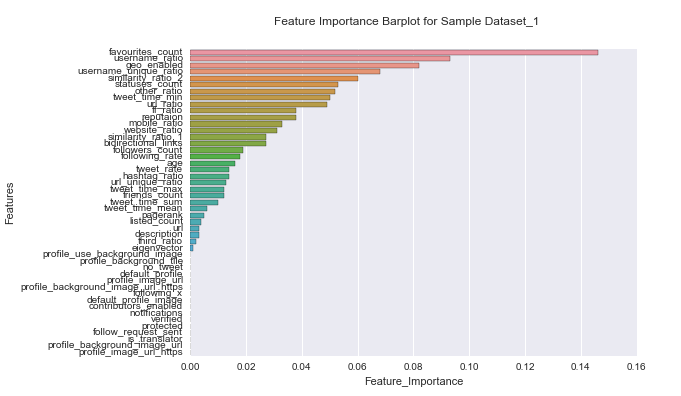
\includegraphics[scale=0.7]{feature_1}
	\caption{Feature Importance}
	\label{fig:mesh1}
\end{figure}



\noindent Lastly, we used confusion matrix to check the accuracy of the random forest model. In order to better visualize and interpret the results, we used the normalized confusion matrix so that the ratio is at the same scale. Figure 2 shows that fake accounts have higher prediction accuracy score, in which indicates that the model did a better job in predicting fake accounts than genuine accounts for sample dataset 1. 

\begin{figure}[H]
	\centering
	\begin{subfigure}{.5\textwidth}
		\centering
		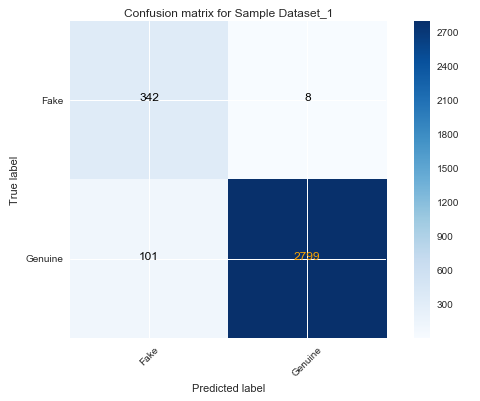
\includegraphics[scale=0.6]{matrix_1}
		\caption{Without Normalization}
		\label{fig:sub1}
	\end{subfigure}%
	\begin{subfigure}{.5\textwidth}
		\centering
		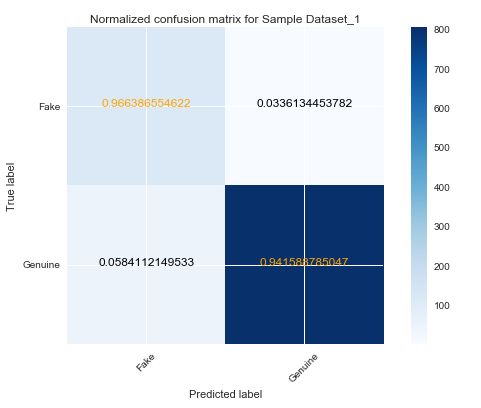
\includegraphics[scale=0.6]{matrix_nor_1}
		\caption{With Normalization}
		\label{fig:sub2}
	\end{subfigure}
	\caption{Confusion Matrix}
\end{figure}

\section{Conclusion/Insights}

\section{Future}
Here are some possible directions that we are considering for the next step:

\noindent 1. Create more features in predicting the account type\\
2. Further evaluate the models that we built and use methods to reduce noise and errors\\
3. Investigate on other models that we can potentially use\\
4. Create an interactive platform to allow the Twitter users to use our predictive models\\


\section{Appendix}
\subsection{Reflection}
Overall, we had successfully accomplished the goal of our project, in which allows the Twitter users to identify whether the account is fake or genuine using Random Forest, Logistic Regression and Support Vector Machine. We were unable to analyze the fake users' behaviors on the trend topics due to the time constraint. Each group member was assigned to build different features and predictive models. All of us had contributed equally. We met regularly to check on each other's progress and discuss the problems that we had encountered. Since each of us has very different levels of skill sets and knowledge, it was challenging to include and implement everyone's initial ideas. However, we were able to compromise and find common interests through discussions. Originally, we wanted to analyze all the tweets that the user has posted. However, the Twitter API has set limit on the amount of info that we could get. Therefore, we only downloaded the maximum number of tweets that we were allowed. In addition, we were planning to build features on predicting twitter account types from the scratch. However, we had realized that it is important to conduct research on previous studies and use them as references. \\

\noindent As the project progressed, we narrowed down the models that we wanted to build and try to understand the math and concepts behind them, We learned that it is important to create a feasible time-line for any project because it is often easy to overestimate the amount of work that we think we can accomplish. In addition, we need to understand the context of the data, the intuitions behind the models and how our analysis can help answer the questions that we want to solve.\\
\subsection{Code Appendix}
* random\_forest.py - builds random forest model\\
* t\_analysis.py - calculates tweet analysis ratios\\
* similarity\_1.py - calculates tweet similarity ratio 1\\
* similarity\_2.py - calculates tweet similarity ratio 2\\
* tweet\_ratio.py - creates a csv file that contains the tweet analysis ratios\\
* sim\_1\_df.py - creates a csv file for storing the tweet similarity ratio 1 result\\
* sim\_2\_df.py - creates a csv file for storing the tweet similarity ratio 2 result\\
* combine\_df.py - combines all the feature results into a dataframe\\
* tweet\_time\_diff.py - calculates the time difference between two consecutive tweets\\

\section{Reference}
[1]O.Varol, E.Ferrara, C.A.Davis, F.Menczer, and A.Flammini. Online Human-Bot Interactions: Detection, Estimation, and Characterization\\

\noindent [2] F. Benevenuto, G. Magno, T. Rodrigues, and V. Almeida. Detecting Spammers on Twitter. In Collaboration, Electronic messaging, Anti-Abuse and Spam Confference.\\

\noindent [3] K. Lee, J. Caverlee, and S. Webb. Uncovering Social Spammers: Social Honeypots Machine Learning. In ACM SIGIR Conference (SIGIR), 2010.\\

\noindent [4] G. Stringhini, S. Barbara, C. Kruegel, and G. Vigna. Detecting Spammers On Social Networks. In Annual Computer Security Applications Conference (ACSAC’10), 2010.\\

\noindent [5] A. Wang. Don’t follow me: spam detecting in Twitter. In Int’l Conferene on Security and Cryptography (SECRYPT), 2010.\\

\noindent [6] G. Stringhini, C. Kruegel, G. Vigna Detecting Spammers on Social Networks\\

\noindent [7] C. Yang, R. Harkreader, and G. Gu. Empirical evaluation and new design for fighting evolving Twitter spammers. I.\\

\noindent [8] Nando de Freitas. "Machine learning - Random forests." Online video clip. YouTube. YouTube, 21 Feb 2013


\end{document}